%CONFIGURACIÓN DEL DOCUMENTO Y HOJA

\documentclass[11pt,letterpaper]{article}
\setlength{\parindent}{0em}                  %DISTANCIA SANGRÍA
\setlength{\parskip}{0.5em}                  %DISTANCIA ENTRE PÁRRAFOS
\textwidth 6.5in
\textheight 9.in
\oddsidemargin 0in
\headheight 0in

%PAQUETES DEL TEMPLATE

\usepackage{fancybox}
\usepackage[utf8]{inputenc}
\usepackage{epsfig,graphicx}
\usepackage{multicol,pst-plot}
\usepackage{pstricks}
\usepackage{amsmath}
\usepackage{amsfonts}
\usepackage{amssymb}
\usepackage{eucal}
\usepackage[left=2cm,right=2cm,top=2cm,bottom=2cm]{geometry}
\usepackage{txfonts}
\usepackage[spanish]{babel}
\usepackage[colorlinks]{hyperref}
\usepackage{cancel}
\usepackage{caption}
\usepackage{float}
\usepackage{upgreek}
\usepackage{gensymb}
\usepackage{subfigure}
\usepackage{siunitx}
\usepackage{color}
\usepackage{tikz}
\usepackage{listings}

\usepackage{mdframed}
\usepackage[
backend=bibtex,
style=ieee,
sorting=none
]{biblatex}
\addbibresource{biblio.bib}
\usepackage{multicol}
\usepackage{stackrel}

%DEFINICIÓN DE COLORES EXTRAS

\definecolor{codegreen}{rgb}{0,0.6,0}
\definecolor{codegray}{rgb}{0.5,0.5,0.5}
\definecolor{backcolour}{rgb}{0.95,0.95,0.95}
\hypersetup{colorlinks=true,linkcolor=codegreen,citecolor=blue,filecolor=blue,urlcolor=magenta,}

%CONFIGURACIÓN DE LSTLISTINGS PARA CÓDIGOS

\lstset{ %
language=python,                % choose the language of the code
basicstyle=\footnotesize,       % the size of the fonts that are used for the code
numbers=left,                   % where to put the line-numbers
numberstyle=\footnotesize,      % the size of the fonts that are used for the line-numbers
stepnumber=1,                   % the step between two line-numbers. If it is 1 each line will be numbered
numbersep=5pt,                  % how far the line-numbers are from the code
backgroundcolor=\color{white},  % choose the background color. You must add \usepackage{color}
showspaces=false,               % show spaces adding particular underscores
showstringspaces=false,         % underline spaces within strings
showtabs=false,                 % show tabs within strings adding particular underscores
frame=single,                   % adds a frame around the code
tabsize=2,                      % sets default tabsize to 2 spaces
captionpos=b,                   % sets the caption-position to bottom
breaklines=true,                % sets automatic line breaking
breakatwhitespace=false,        % sets if automatic breaks should only happen at whitespace
escapeinside={\%*}{*)}          % if you want to add a comment within your code
}
\lstdefinestyle{mystyle}{
	backgroundcolor=\color{backcolour},
	commentstyle=\color{red},
	keywordstyle=\bfseries\color{magenta},
	numberstyle=\tiny\color{codegray},
	stringstyle=\color{codegreen},
	basicstyle=\footnotesize\ttfamily,
	identifierstyle=\color{blue},
	breakatwhitespace=false,
	breaklines=true,
	captionpos=b,
	keepspaces=true,
	numbers=left,
	numbersep=5pt,
	showspaces=false,
	showstringspaces=false,
	showtabs=false,
	tabsize=2
}

\lstset{style=mystyle}

%CONFIGURACIÓN DE MINTED PARA CÓDIGOS



%DEFINICIÓN DE COMANDOS EXTRAS

\pagestyle{empty}
\newcommand{\units}[1]{\left[ #1 \right]}          %CORCHETES PARA UNIDADES
\newcommand{\abs}[1]{\left|#1\right|}              %OPERADOR VALOR ABSOLUTO INTEGRALES

%COMIENZA EL DOCUMENTO

\begin{document}

%CONFIGURACIÓN DEL ENCABEZADO

\usetikzlibrary{positioning}
\tikzset{every picture/.style={line width=0.75pt}}
\pagestyle{plain}
\begin{flushleft}
Ingeniería de la Salud \hfill Bioinformática\\
Escuela Técnica Superior de Ingeniería Informática\\
\underline{Universidad de Málaga}
\end{flushleft}

\begin{flushright}\vspace{-5mm}

\includegraphics[height=1.5cm]{escudo.jpg}
\end{flushright}

\begin{center}\vspace{-1cm}
\textbf{\large Práctica 5. Reordenación del Genoma.}\\   %TITULO
Arrabalí Cañete, Carmen Lucía\\                         %NOMBRE
\end{center}
\rule{\linewidth}{0.1mm}

%DESDE AQUÍ SE ESCRIBE TODO EL CONTENIDO

\section{Introducción y objetivos}
Los reordenamientos del genoma describen cambios en la relación de enlace genético de grandes regiones cromosómicas, que implican inversiones, transposiciones, intercambios de bloques, deleciones, inserciones, fusiones y translocaciones, etc.

En este caso, el objetivo principal es estudiar e implementar los algoritmos de ordenación de permutaciones como son los algoritmos \texttt{prefix sort}, algoritmo de fuerza bruta, y \texttt{break point reversal}, algoritmo voraz.

\subsection{Contexto Biológico del problema}
Los genes son secuencias de nucleótidos que codifican la síntesis de material bioquímico (ya sea ARN o proteínas).
Los procesos biológicos pueden dar lugar a mutaciones en el genoma. Algunas son locales y afectan a un solo nucleótido (sustituciones inserciones, deleciones) mientras que otras pueden ser no locales y afectar a largos tramos de la secuencia (inversiones, transposiciones, translocaciones). Las mutaciones no locales son raras, pero se acumulan a lo largo de la evolutiva. Por lo tanto, son un buen indicador de la distancia evolutiva entre especies.

\section{Planteamiento del problema. El genoma como permutación}
Se deja que el orden de los genes en un organismo se represente como una permutación con signo. Denominando a las permutaciones como $\pi = \left [ \pi_1 \pi_2 ... \pi_n \right ]$

También hay que tener en cuenta las restricciones en cuanto a la orientación de los genes:

\begin{itemize}
	\item Si la orientación de los genes no es importante, cada $\pi_i \in \left \{ 1, 2, ..., n \right \}$ es un número entero positivo no repetido.
	\item Si la orientación del gen es importante, cada $\pi_i$ puede ser positivo o negativo, y $\left |\pi_i\right | \in \left \{ 1, 2, ..., n \right \}$ es un número entero positivo no repetido positivo no repetido.
\end{itemize}

\subsection{Reversal}

Una inversión $\rho (i, j)$ es una operación que afecta a la parte del genoma entre las posiciones i y j (ambas inclusive), invirtiendo este segmento.

\subsection{Minimal Reversal Distance}

Sean $\pi$ y $\pi^{'}$ dos organismos. La distancia de inversión entre es el número mínimo de inversiones necesarias para transformar una de las permutaciones en la otra.
Se puede suponer, por ejemplo, que una de las permutaciones, $\pi^{'}$ es la permutación de identidad positiva, es decir, $\pi^{'}_i = 1$, $1 \leqslant i \leqslant n $.

\section{Configuración del equipo}
Se ha realizado la implementación en un equipo con un sistema operativo Windows 10 Home 64 bits, con un procesador Intel$($R$)$ Core $($TM$)$ i7-6500U CPU $@$ 2.50GHz 2.59 GHz $($4 CPUs$)$ y un disco SSD de 480GB y 12GB de RAM. La versión Java corresponde a la número 17.

\section{Implemetación}
\subsection{Clase PrefixSort.java}
En el método principal, \textit{protected void \_run(Permutation l)}, se implementa PrefixSort, el cual se encarga de ordenar la secuencia, ver apartado~\ref{ch:31}, recibe como parámetro una permutación, cuya longitud tiene que ser mayor que la unidad. Por otro lado, la  permutación como tal no puede ser la identidad (método ya creado) y cuya posición i no puede ser i+1.

Se le aplica el método \texttt{Reversal} y se incrementa el número de operaciones totales para así saber cual es el total de permutaciones que realiza el algoritmo.

\subsubsection{Método \textit{protected void \_run(Permutation l)} de la clase \textit{PrefixSort.java}}\label{ch:31}

\begin{lstlisting}[language = java]
	protected void _run(Permutation l) {
		int n = l.size();
		for(int i=0; i<n; i++) {
			if(n > 1 && !l.isIdentity() && l.get(i) != i+1) {
				int j = l.indexOf(i+1);
				Reversal p = new Reversal(i, j);
				p.apply(l);
				numOperations++;
			}
		}
	}
\end{lstlisting}

\subsection{Clase BreakpointReversalAlgorithm.java}
En el primer método de la implementación, \textit{protected List<SequenceRearrangementOperation> getCandidates(Permutation p)} (ver apartado ~\ref{ch:32}) recibe como parámetro los candidatos posibles que pueden realizar una permutación y son aquellos que entre si mismo y el siguiente valor de la cadena de estudio haya más de 1 de diferencia. En el caso de que no sea así, se considera como no candidato puesto que ya estaría ordenado. En primer lugar se encuentran los puntos de ruptura y luego se evalúan para comprobar que es un candidato factible.

En el segundo método de esta clase, \textit{protected double getOperationQuality(Permutation p, SequenceRearrangementOperation op)}, se trata de buscar, entre todos los candidatos posibles, el que sea de mayor calidad. Esto quiere decir que, en el caso de tener una permutación que consiga eliminar 2 breakpoints y otra permutación que elimine 1 solo, se cogerá el que consiga eliminar los 2 puesto que será de mayor calidad.

\subsubsection{Método \textit{protected List<SequenceRearrangementOperation> getCandidates(Permutation p)} de la clase \textit{BreakpointReversalAlgorithm.java}}\label{ch:32}
\begin{lstlisting}[language = java]
	protected List<SequenceRearrangementOperation> getCandidates(Permutation p) {
		int n = p.size();
		List<SequenceRearrangementOperation> ops = new LinkedList<SequenceRearrangementOperation>();
		
		// 1) Find where the breakpoints are.
		int[] breakpoints = new int[n];
		int numBP = 0;
		for (int i = 0; i < n-1 ; i++) {
			if (Math.abs(p.get(i)-p.get(i+1)) > 1) {				
				breakpoints[numBP] = i;
				numBP++;
			}
		}
			
		// 2) Candidates are reversals between breakpoints.
		for (int i = 0; i < numBP; i++) {
			for (int j = i+1; j < numBP; j++) {
				ops.add(new Reversal(breakpoints[i]+1,breakpoints[j]));				
			}
		}
		return ops;
	}
	
\end{lstlisting}

\subsubsection{Método \textit{protected double getOperationQuality(Permutation p, SequenceRearrangementOperation op)} de la clase \textit{BreakpointReversalAlgorithm.java}}\label{ch:33}
\begin{lstlisting}[language = java]
	protected double getOperationQuality(Permutation p, SequenceRearrangementOperation op) {
		Reversal r = (Reversal) op;
		int result = 0;
		
		if (Math.abs(p.get(r.getStart()-1)  - p.get(r.getFinish()) ) == 1) {
			result++;
		}
		if (Math.abs(p.get(r.getFinish()+1)  - p.get(r.getStart()) ) == 1) {
			result++;
		} 
		return (double) result;
	}
	
\end{lstlisting}


\section{Resultados y Conclusiones}
Para poder analizar correctamente los resultados, el método main recibe en los argumentos de entrada, varios modos de ejecución entre los que se encuentra \textit{$-$r $<$algorithm$>$ $<$init\_length$>$ $<$doubling$>$ $<$num\_test$>$} el cual genera un archivo con permutaciones aleatorias con distintas longitudes. La longitud inicial de las permutaciones viene dada por init\_length, y se irá aumentando la longitud tantas veces como indique el parámetro doubling. Todas las permutaciones se ordenarán con el algoritmo que se pasa como primer parámetro.

Al utilizar ese modo de ejecución, se genera un archivo con los diferentes tiempos de ejecución, el cual se llama  un archivo \textit{PrefixSortrearrangement.txt} y \textit{BreakpointReversalrearrangement.txt}

Por otro lado, entre los recursos aportados en el Campus Virtual se tiene un archivo llamado \textit{analyze.R} que contiene un script el cual se encarga de generar una gráfica para cada algoritmo haciendo uso de los archivos .txt generados anteriormente con el modo de ejecución $-$r.
\begin{multicols}{2}
	\begin{figure}[H]
		\centering
		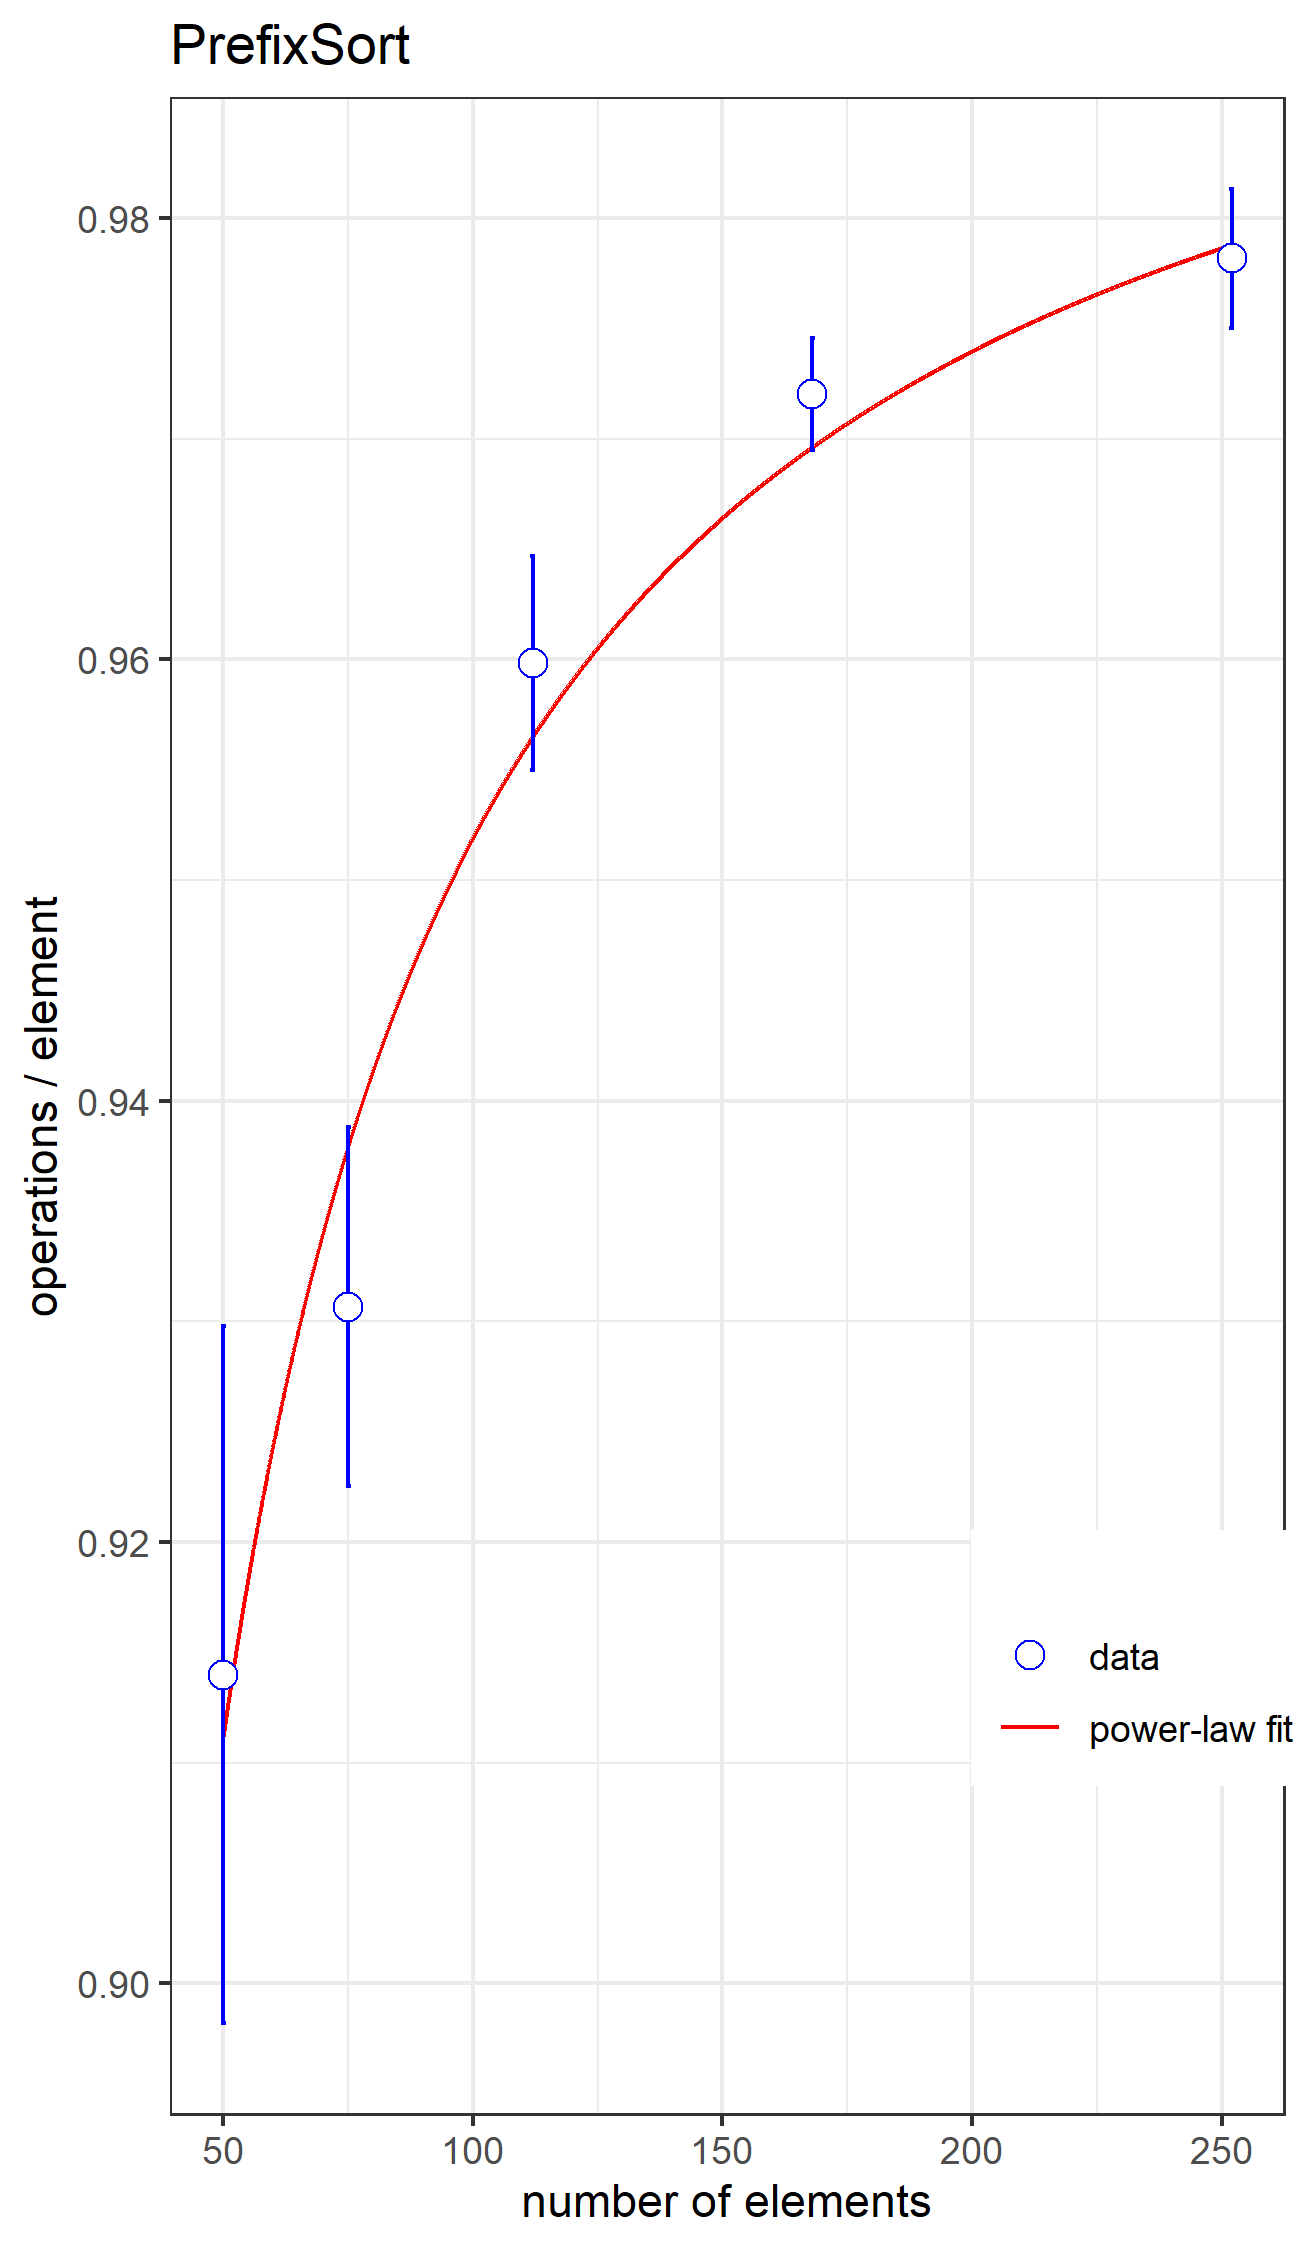
\includegraphics[width=0.4\textwidth]{img/PrefixSort.png}
		\caption{Resultado de la ejecución del algoritmo PrefixSort con los parámetros utilizados.}
		\label{fig:graficoPS}
	\end{figure}
	
	\begin{figure}[H]
		\centering
		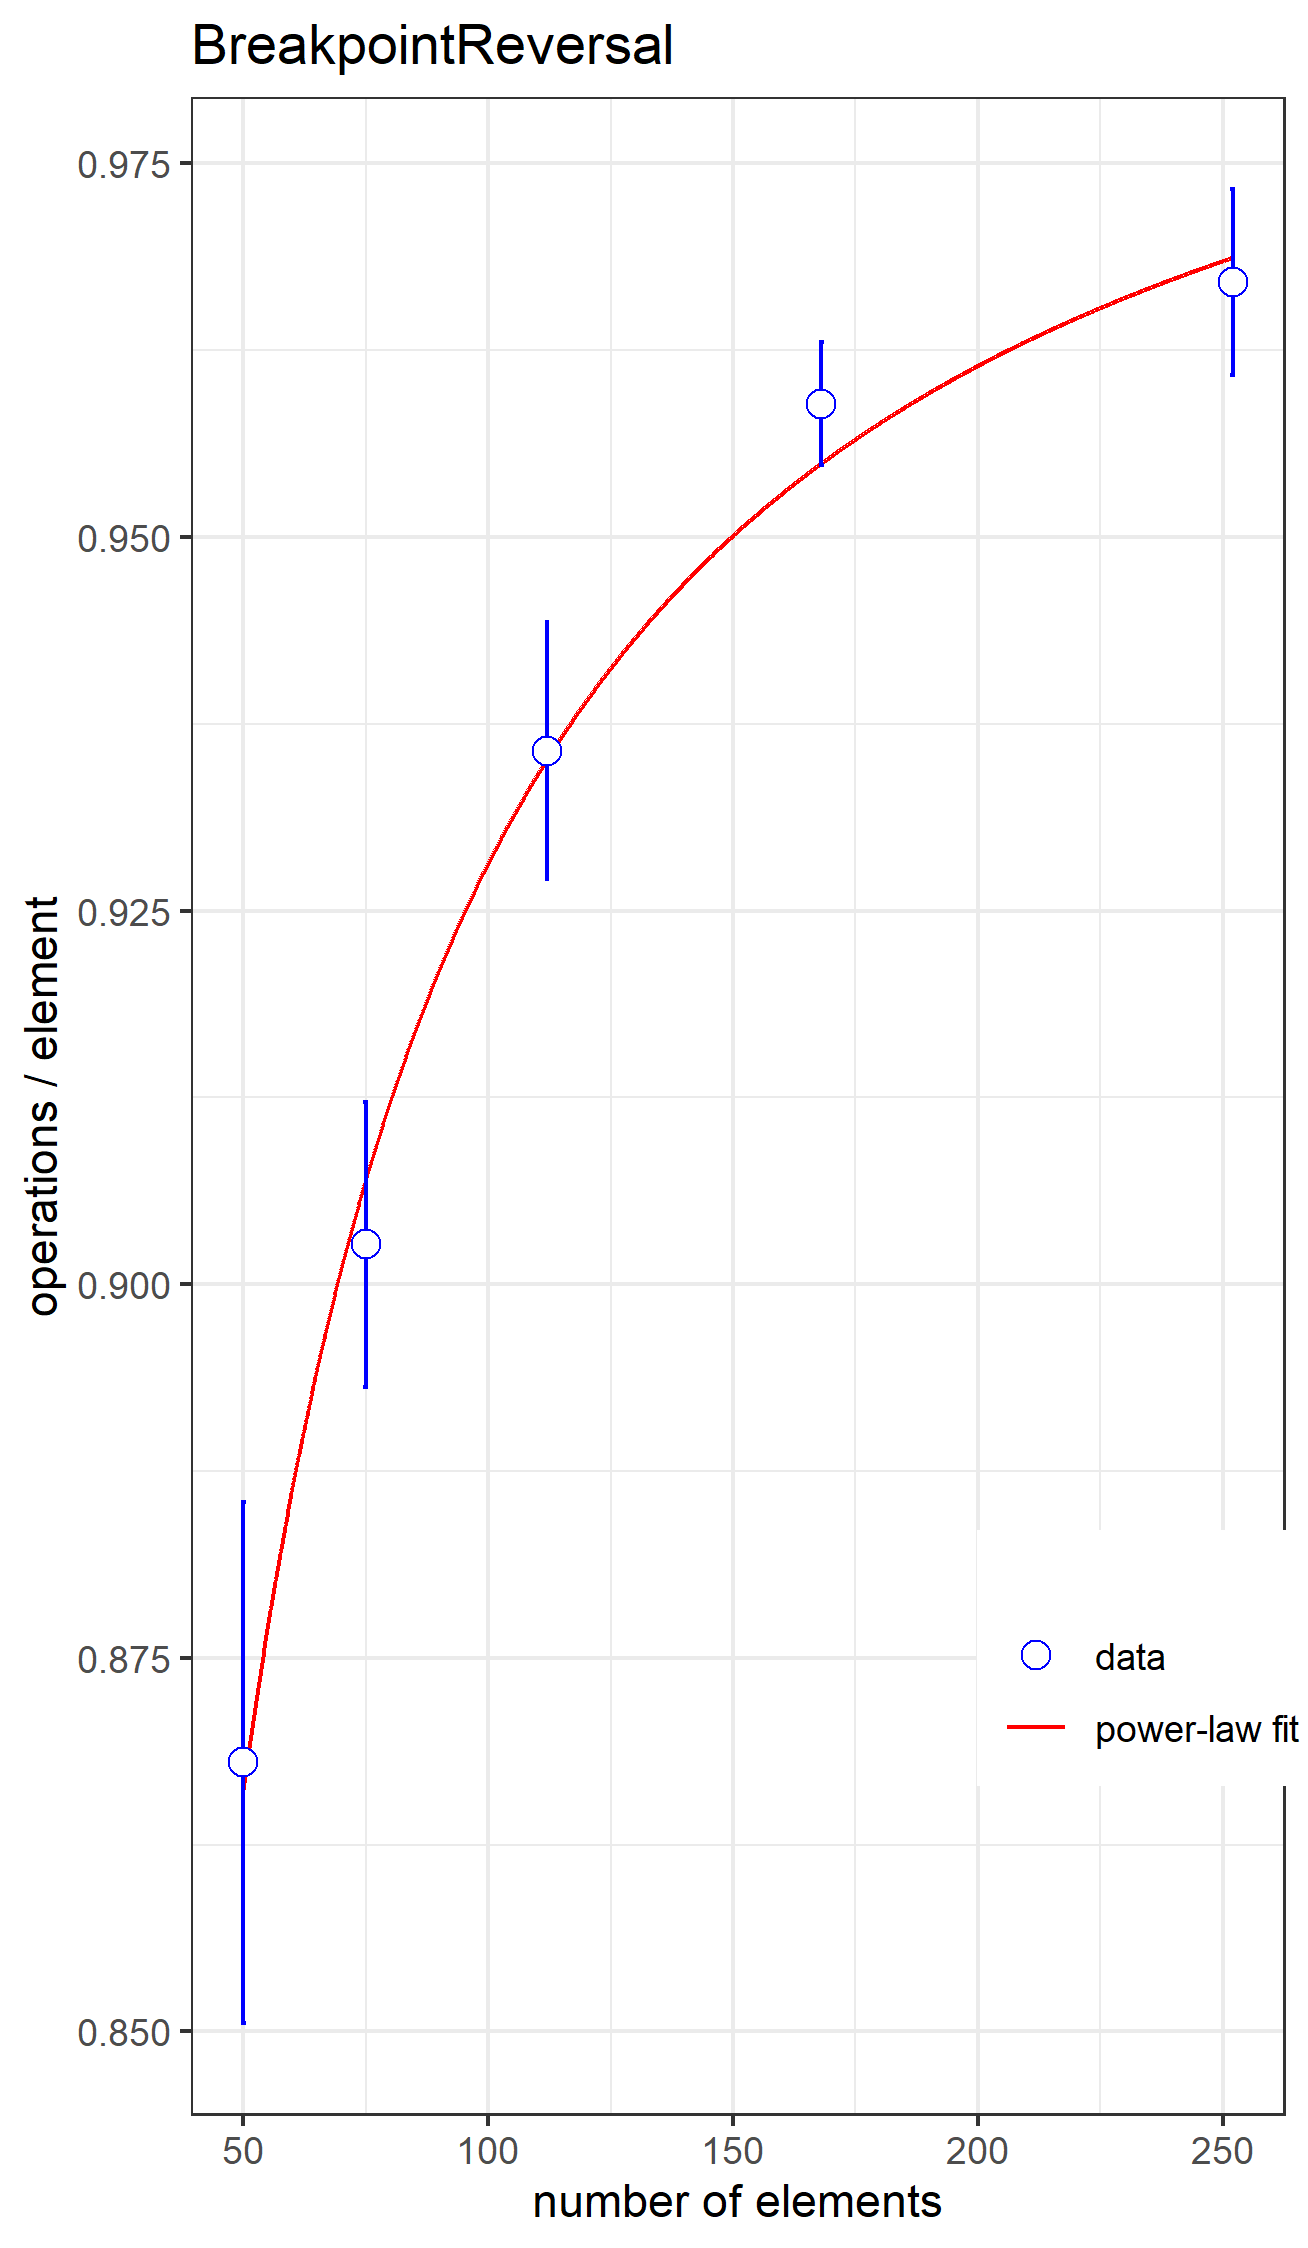
\includegraphics[width=0.4\textwidth]{img/BreakpointReversal.png}
		\caption{Resultado de la ejecución del algoritmo BreakpointReversal con los parámetros utilizados.}
		\label{fig:graficoBPR}
	\end{figure}
	
\end{multicols}

Para poder generar un archivo con unos datos asequibles para el algoritmo y para el equipo que se utiliza, se han dado los siguientes valores: 

\begin{multicols}{2}
	\begin{itemize}
		\item \textbf{$<$algoritmo$>$}: PrefixSort o BreakPointReversal
		\item \textbf{$<$init\_length$>$}: 50
		\item \textbf{$<$doubling$>$}: 5
		\item \textbf{$<$num\_test$>$}: 10
	\end{itemize}
\end{multicols}

Como se puede observar en las figuras~\ref{fig:graficoPS} y~\ref{fig:graficoBPR}, cuanto mayor sea el número de elementos de la cadena con la que se quiere obtener el reordenamiento, el número de operaciones que tiene que realizar el algoritmo es mayor, por lo que tiene un coste más elevado. 

\end{document}
